\definecolor{designblue}{RGB}{222,236,248}
\definecolor{creambox}{RGB}{255,247,232}

\setlength{\tabcolsep}{3pt}
\renewcommand{\arraystretch}{1.2}

\heading{Design Choices}
This section summarizes the principal modeling and solver choices adopted in the verifier.

\begin{itemize}
  \item \textbf{CHC semantics with Z3 Fixedpoint/SPACER:} Program behavior is encoded as CHCs and solved using Z3 \texttt{Fixedpoint} with \texttt{engine='spacer'} (an IC3/PDR-style Horn-clause engine), with safety posed as \texttt{Exists(s, Inv(s) \& Not(P(s)))}.
  \item \textbf{Single global invariant schema:} A unified relation \texttt{Inv(pc, xcor, ycor, heading, pendown, user\_vars, loop\_counters)} is used across initialization, transition rules, and property queries.
  \item \textbf{Heading-lattice geometry model:} Heading is normalized to \texttt{[0,360)} and constrained to \texttt{\{0,15,\dots,345\}}, with violations represented explicitly via \texttt{BadHeading}.
\end{itemize}

\begin{table}
\centering
\begin{tabular}{
  >{\raggedright\arraybackslash\columncolor{designblue}}p{0.25\linewidth}
  p{0.34\linewidth}
  p{0.35\linewidth}
}
\rowcolor{designblue}
\textbf{Design Choice} & \textbf{Benefit} & \textbf{Tradeoff} \\

\textbf{CHCs solved by Z3 SPACER} &
Supports unbounded safety checking through inductive invariant synthesis and returns counterexample witnesses on violation. &
Performance remains sensitive to nonlinear arithmetic obligations; solver outcomes may be \texttt{UNKNOWN}. \\

\textbf{Full state (\texttt{pc}+counters+vars)} &
Encodes control-state and data-state dependencies in one relation: \texttt{pc} for control/termination, \texttt{xcor/ycor/heading} for geometric predicates, and loop counters for repeat constructs. &
Properties over a strict subset of variables still incur full-arity reasoning, increasing solver cost. \\

\textbf{Strict heading lattice + \texttt{BadHeading}} &
Avoids direct transcendental \texttt{sin/cos} constraints in SPACER by using a finite 15-degree trigonometric lookup table (precomputed in Python) with explicit \texttt{BadHeading} obligations. &
Lookup expansion must remain bounded to control CHC size; failure to prove grid preservation yields conservative \texttt{UNKNOWN} outcomes. \\

\end{tabular}
\end{table}

\heading{Optimizations}
{\centering\large\textbf{Turn-Safe Heading Inference}\par}
\noindent
\begin{minipage}[t]{0.48\linewidth}
\centering
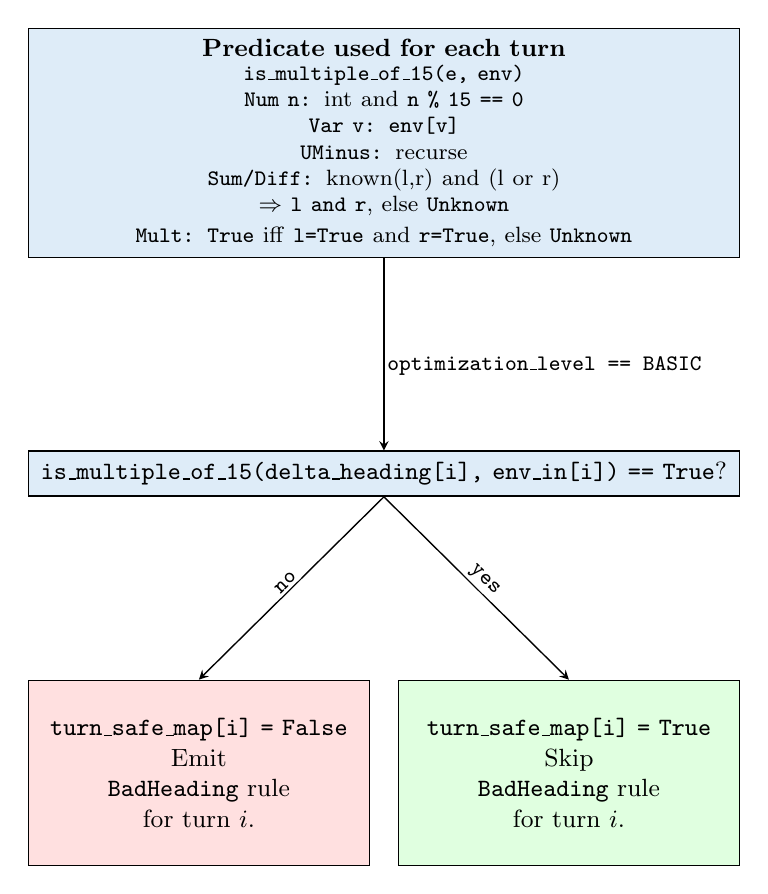
\begin{tikzpicture}[>=stealth, line width=0.5pt, font=\small, baseline=(current bounding box.north)]
\tikzset{
  optkey/.style={draw, align=center, fill=designblue, text width=8.75cm, inner sep=4pt},
  optdec/.style={draw, align=center, fill=designblue, text width=8.75cm, inner sep=4pt},
  optoutno/.style={draw, align=center, fill=red!12, text width=4.05cm, inner sep=4pt, minimum height=2.35cm},
  optoutyes/.style={draw, align=center, fill=green!12, text width=4.05cm, inner sep=4pt, minimum height=2.35cm}
}

\node[optkey] (k1) at (0,0) {\textbf{Predicate used for each turn}\\[-1pt]
{\footnotesize\texttt{is\_multiple\_of\_15(e, env)}\\
\texttt{Num n:} int and \texttt{n \% 15 == 0}\\
\texttt{Var v:} \texttt{env[v]}\\
\texttt{UMinus:} recurse\\
\texttt{Sum/Diff:} known(l,r) and (l or r)\\ $\Rightarrow$ \texttt{l and r}, else \texttt{Unknown}\\
\texttt{Mult:} \texttt{True} iff \texttt{l=True} and \texttt{r=True}, else \texttt{Unknown}}};

\node[optdec] (d1) at (0,-4.2) {\texttt{is\_multiple\_of\_15(delta\_heading[i], env\_in[i]) == True}?};

\node[optoutno] (nL) at (-2.35,-8.0) {\texttt{turn\_safe\_map[i]} \texttt{= False}\\Emit\\\texttt{BadHeading} rule\\for turn $i$.};
\node[optoutyes] (nR) at (2.35,-8.0) {\texttt{turn\_safe\_map[i]} \texttt{= True}\\Skip\\\texttt{BadHeading} rule\\for turn $i$.};

\draw[->] (k1) -- node[pos=0.56, right, fill=white, inner sep=1pt] {\footnotesize \texttt{optimization\_level == BASIC}} (d1);
\draw[->] (d1.south) -- node[midway, above, sloped, fill=white, inner sep=1pt] {\footnotesize \texttt{no}} (nL.north);
\draw[->] (d1.south) -- node[midway, above, sloped, fill=white, inner sep=1pt] {\footnotesize \texttt{yes}} (nR.north);
\end{tikzpicture}
\end{minipage}\hspace{0.5cm}
\begin{minipage}[t]{0.48\linewidth}
\centering
\begin{tikzpicture}[font=\small, line width=0.5pt, baseline=(ex1.north)]
\node[align=left, anchor=north, text width=8.75cm, inner sep=0pt] (ex1) at (0,0) {{\ttfamily
if :u > 0 [\\
\hspace*{1.2em}:t = 30\\
] else [\\
\hspace*{1.2em}:t = 45\\
]\\
left :t\\
forward 20}};
\end{tikzpicture}
\par\vspace{1.0em}
\begin{minipage}[t]{8.75cm}
\raggedright
\begin{tabular}{@{}lll@{}}
\texttt{NONE}  & \textcolor{orange!80!black}{UNKNOWN} & timeout (60\,s) \\
\texttt{BASIC} & \textcolor{green!60!black}{PASSED}  & solve \textbf{0.055\,s} \\
\end{tabular}

\vspace{0.9em}
{\textit{Why:} \texttt{:t} can only be \texttt{30} or \texttt{45}, so both branches stay on the 15-degree heading grid.
The divisibility check \texttt{(n \% 15 == 0)} is resolved statically on numeric literals, without adding extra arithmetic constraints to Z3.
Under BASIC, this turn is marked safe and its \texttt{BadHeading} rule is not emitted.
That shrinks the CHC system and avoids the heading-safety timeout seen in NONE.\par}
\end{minipage}
\end{minipage}

\vspace{0.1em}
{\centering\large\textbf{Repeat-Loop Summarization}\par}
\noindent
\begin{minipage}[t]{0.48\linewidth}
\centering
\begin{tikzpicture}[font=\small, line width=0.5pt, baseline=(ex2.north)]
\node[align=left, anchor=north, text width=8.75cm, inner sep=0pt] (ex2) at (0,0) {{\ttfamily
:b = 0\\
repeat 100 [\\
\hspace*{1.2em}:a = :a + 1\\
\hspace*{1.2em}:b = :b + :a\\
]}};
\end{tikzpicture}
\par\vspace{1.0em}
\begin{minipage}[t]{8.75cm}
\raggedright
\begin{tabular}{@{}lll@{}}
\texttt{NONE}  & \textcolor{green!60!black}{PASSED} & solve \textbf{35.16\,s} \\
\texttt{BASIC} & \textcolor{green!60!black}{PASSED} & solve \textbf{0.063\,s} \\
\end{tabular}

\vspace{0.9em}
{\textit{Why:} BASIC detects this repeat body as summarizable and composes all 100 iterations into one summarized loop effect.
Instead of exploring each loop step through many CHC transitions, the solver reasons over a single compact relation from loop entry to exit.
This drastically reduces search depth and clause churn during solving.
The extra work shifts to build-time summarization, yielding a much faster proof query.\par}
\end{minipage}
\end{minipage}\hfill
\begin{minipage}[t]{0.48\linewidth}
\centering
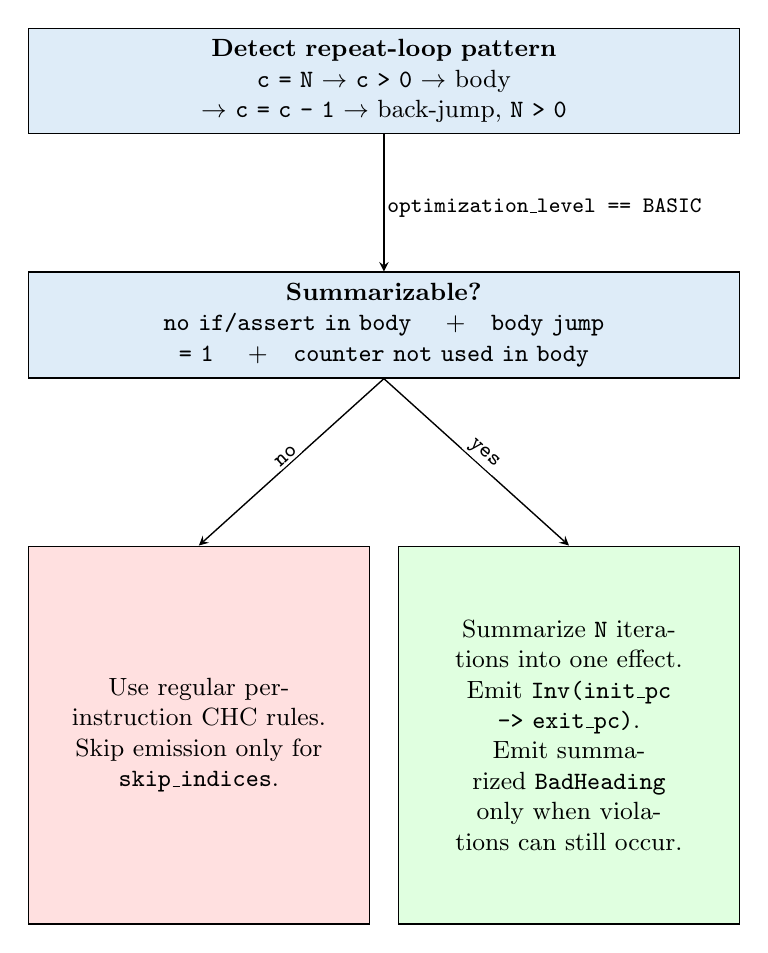
\begin{tikzpicture}[>=stealth, line width=0.5pt, font=\small, baseline=(current bounding box.north)]
\tikzset{
  loopkey/.style={draw, align=center, fill=designblue, text width=8.75cm, inner sep=4pt},
  loopdec/.style={draw, align=center, fill=designblue, text width=8.75cm, inner sep=4pt},
  loopoutno/.style={draw, align=center, anchor=north, fill=red!12, text width=4.05cm, inner sep=4pt, minimum height=4.8cm},
  loopoutyes/.style={draw, align=center, anchor=north, fill=green!12, text width=4.05cm, inner sep=4pt, minimum height=4.8cm}
}

\node[loopkey] (r1) at (0,0) {\textbf{Detect repeat-loop pattern}\\
\texttt{c = N} $\rightarrow$ \texttt{c > 0} $\rightarrow$ body\\
$\rightarrow$ \texttt{c = c - 1} $\rightarrow$ back-jump,\ \texttt{N > 0}};

\node[loopdec] (r2) at (0,-3.1) {\textbf{Summarizable?}\\
\texttt{no if/assert in body} \quad+\quad \texttt{body jump = 1} \quad+\quad \texttt{counter not used in body}};

\node[loopoutno] (rL) at (-2.35,-5.9) {
Use regular per-instruction CHC rules.\\
Skip emission only for\\
\texttt{skip\_indices}.};
\node[loopoutyes] (rR) at (2.35,-5.9) {
Summarize \texttt{N} iterations into one effect.\\
Emit \texttt{Inv(init\_pc -> exit\_pc)}.\\
Emit summarized \texttt{BadHeading}\\
only when violations can still occur.};

\draw[->] (r1) -- node[pos=0.54, right, fill=white, inner sep=1pt] {\footnotesize \texttt{optimization\_level == BASIC}} (r2);
\draw[->] (r2.south) -- node[midway, above, sloped, fill=white, inner sep=1pt] {\footnotesize \texttt{no}} (rL.north);
\draw[->] (r2.south) -- node[midway, above, sloped, fill=white, inner sep=1pt] {\footnotesize \texttt{yes}} (rR.north);
\end{tikzpicture}
\end{minipage}
